% !TEX encoding = UTF-8 Unicode
\documentclass[11pt]{article} % use larger type; default would be 10pt

%%% PAGE DIMENSIONS
\usepackage{geometry} % to change the page dimensions
\geometry{a4paper} % or letterpaper (US) or a5paper or....


%%% PACKAGES
\usepackage[utf8]{inputenc} % set input encoding (not needed with XeLaTeX)
\usepackage{subfiles}
\usepackage{amssymb}
\usepackage{tabulary}
\usepackage{color, colortbl}
\usepackage{xcolor}


\usepackage{graphicx, wrapfig} % support the \includegraphics command and options

\DeclareGraphicsExtensions{.png,.jpg}
\graphicspath{{img/}{../img/}}
\usepackage{gensymb}
\usepackage{pdfpages}
\usepackage{standalone}
\usepackage{float}
\usepackage[toc,page]{appendix}

%%% Codes
\usepackage{listings}
\definecolor{Gray}{gray}{0.9}
\setlength{\parindent}{0em} 

\usepackage[breaklinks=true]{hyperref}


%%% HEADERS & FOOTERS
\usepackage{fancyhdr}	% This should be set AFTER setting up the page geometry
\pagestyle{fancy}	% options: empty , plain , fancy
\renewcommand{\headrulewidth}{0pt}	% customise te layout...
\lhead{}\chead{}\rhead{}
\lfoot{}\cfoot{\thepage}\rfoot{}

%%% END Article customizations

\begin{document}

\begin{titlepage}
    \begin{center}
        \vspace*{1cm}
        
        \Huge
        \textbf{WODSS}
        
        \vspace{0.5cm}
        \LARGE
        Event Planner
      
        \vspace{1.5cm}
        
        \textbf{Autoren: Andreas Gassmann, Jonas Frehner, Lukas Schönbächler}\\

		\vspace{1.5cm}        
                
        \vfill
        
       
        \vspace{0.8cm}
        
        
\includegraphics[width=0.4\textwidth]{title/fhnw}
        
        \Large
        FHNW\\
        Schweiz\\
        März 27, 2017
        
    \end{center}
\end{titlepage}

\begin{abstract}
Das Ziel dieser Arbeit ist die Entwicklung eines Tools welches das Managen von IT-Kolloquien der FHNW erlaubt.
\end{abstract}

\newpage
\tableofcontents
\newpage

\section{Mockups}
\subsection{Login}
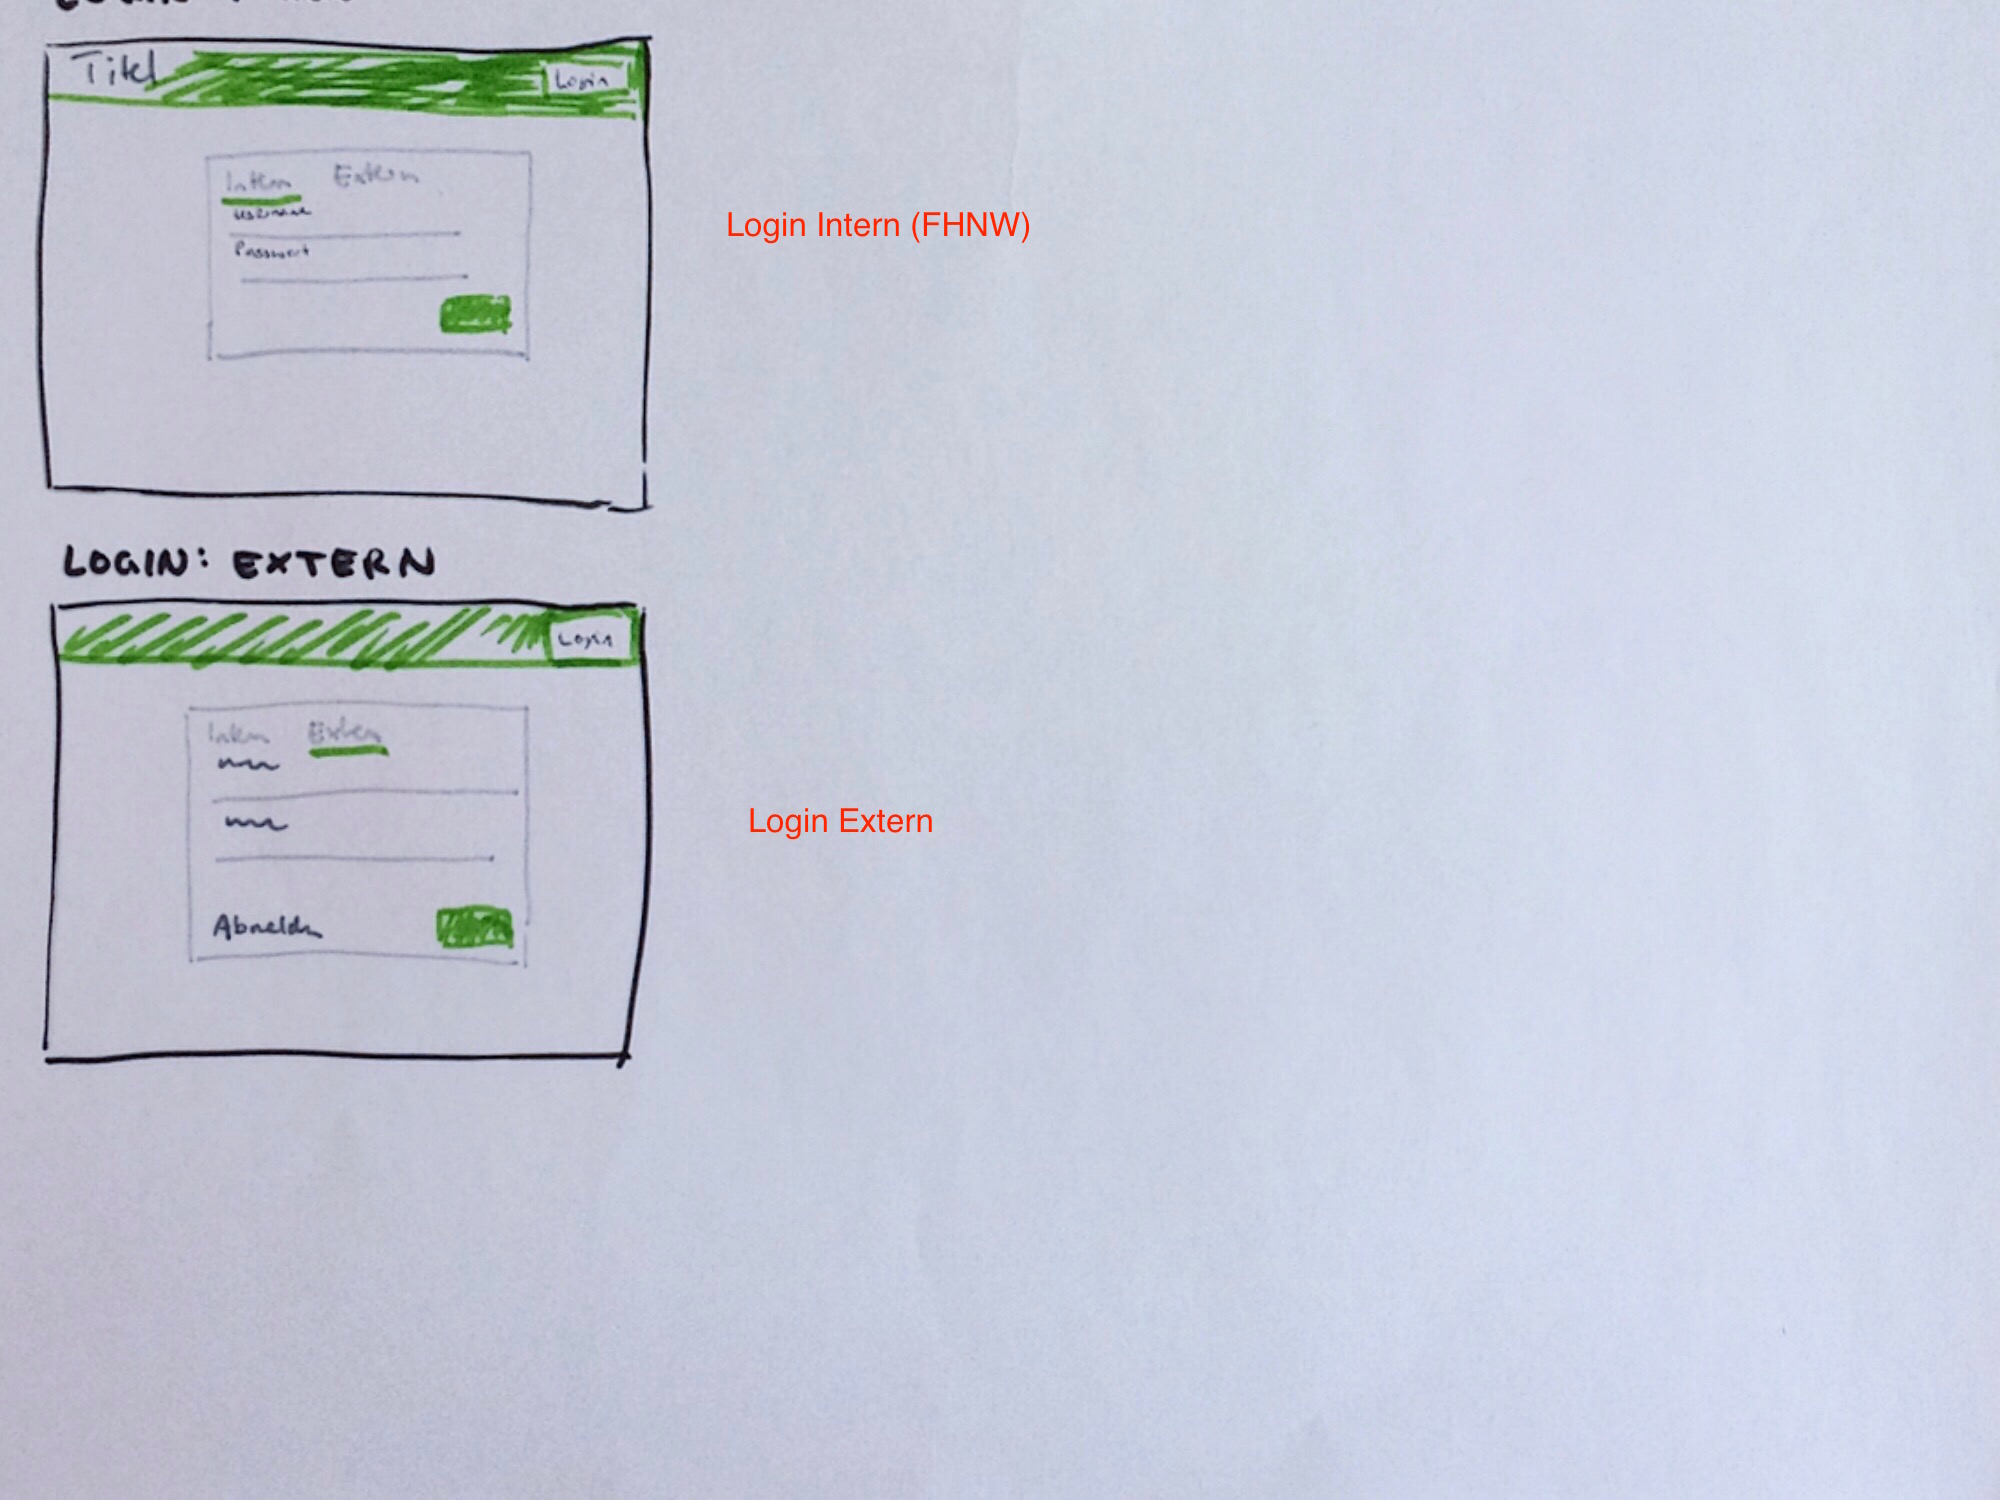
\includegraphics[width=1\textwidth]{prototyp/Login}

\subsection{Übersicht}
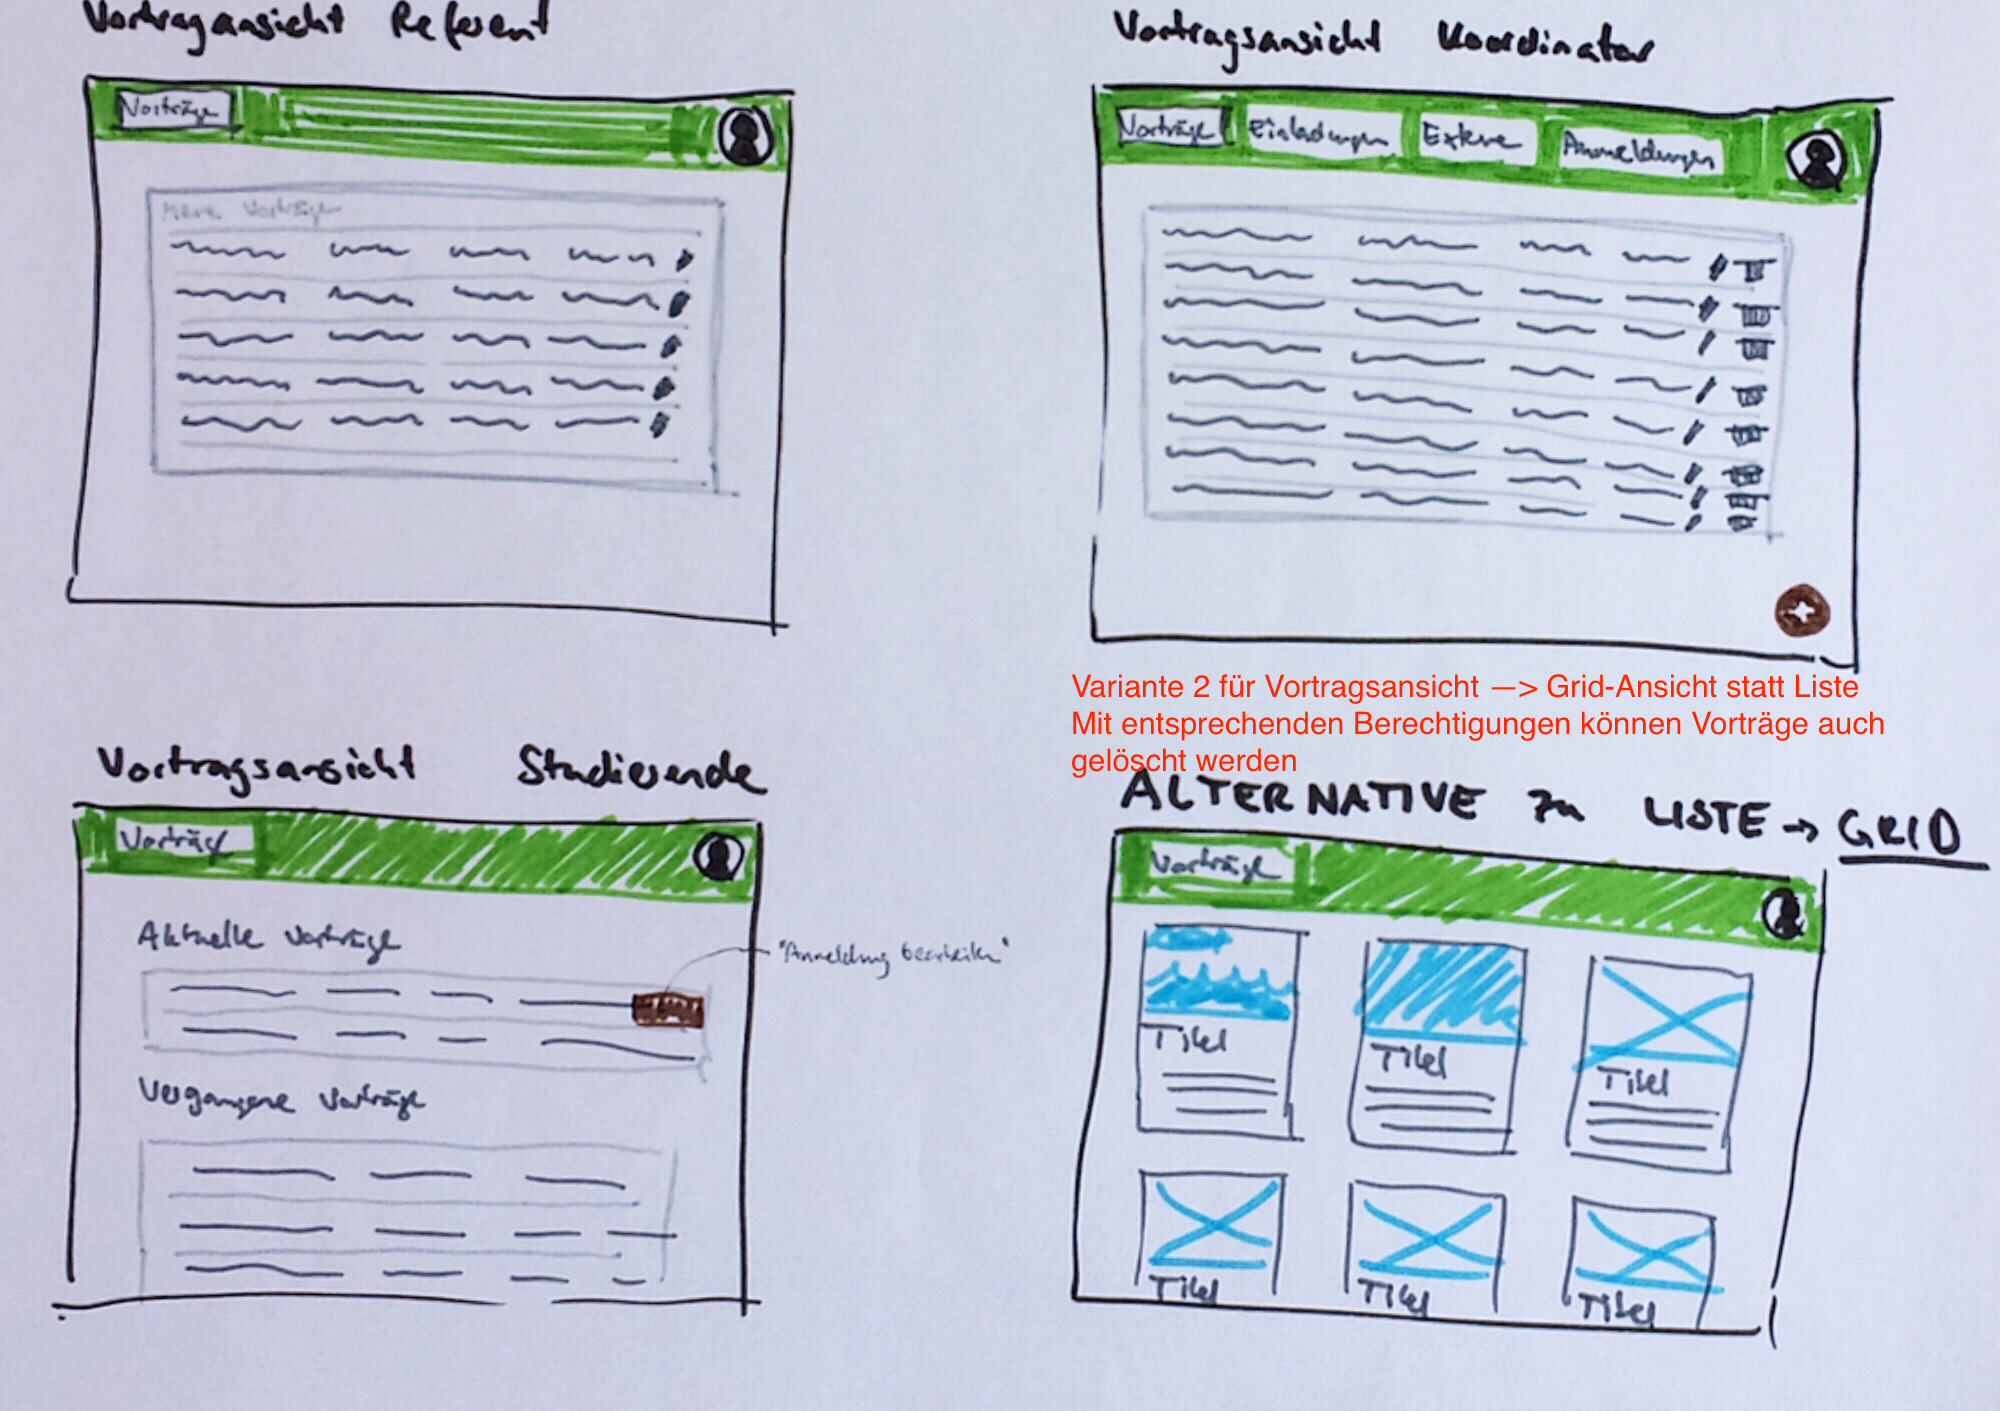
\includegraphics[width=1\textwidth]{prototyp/Vortragansicht}
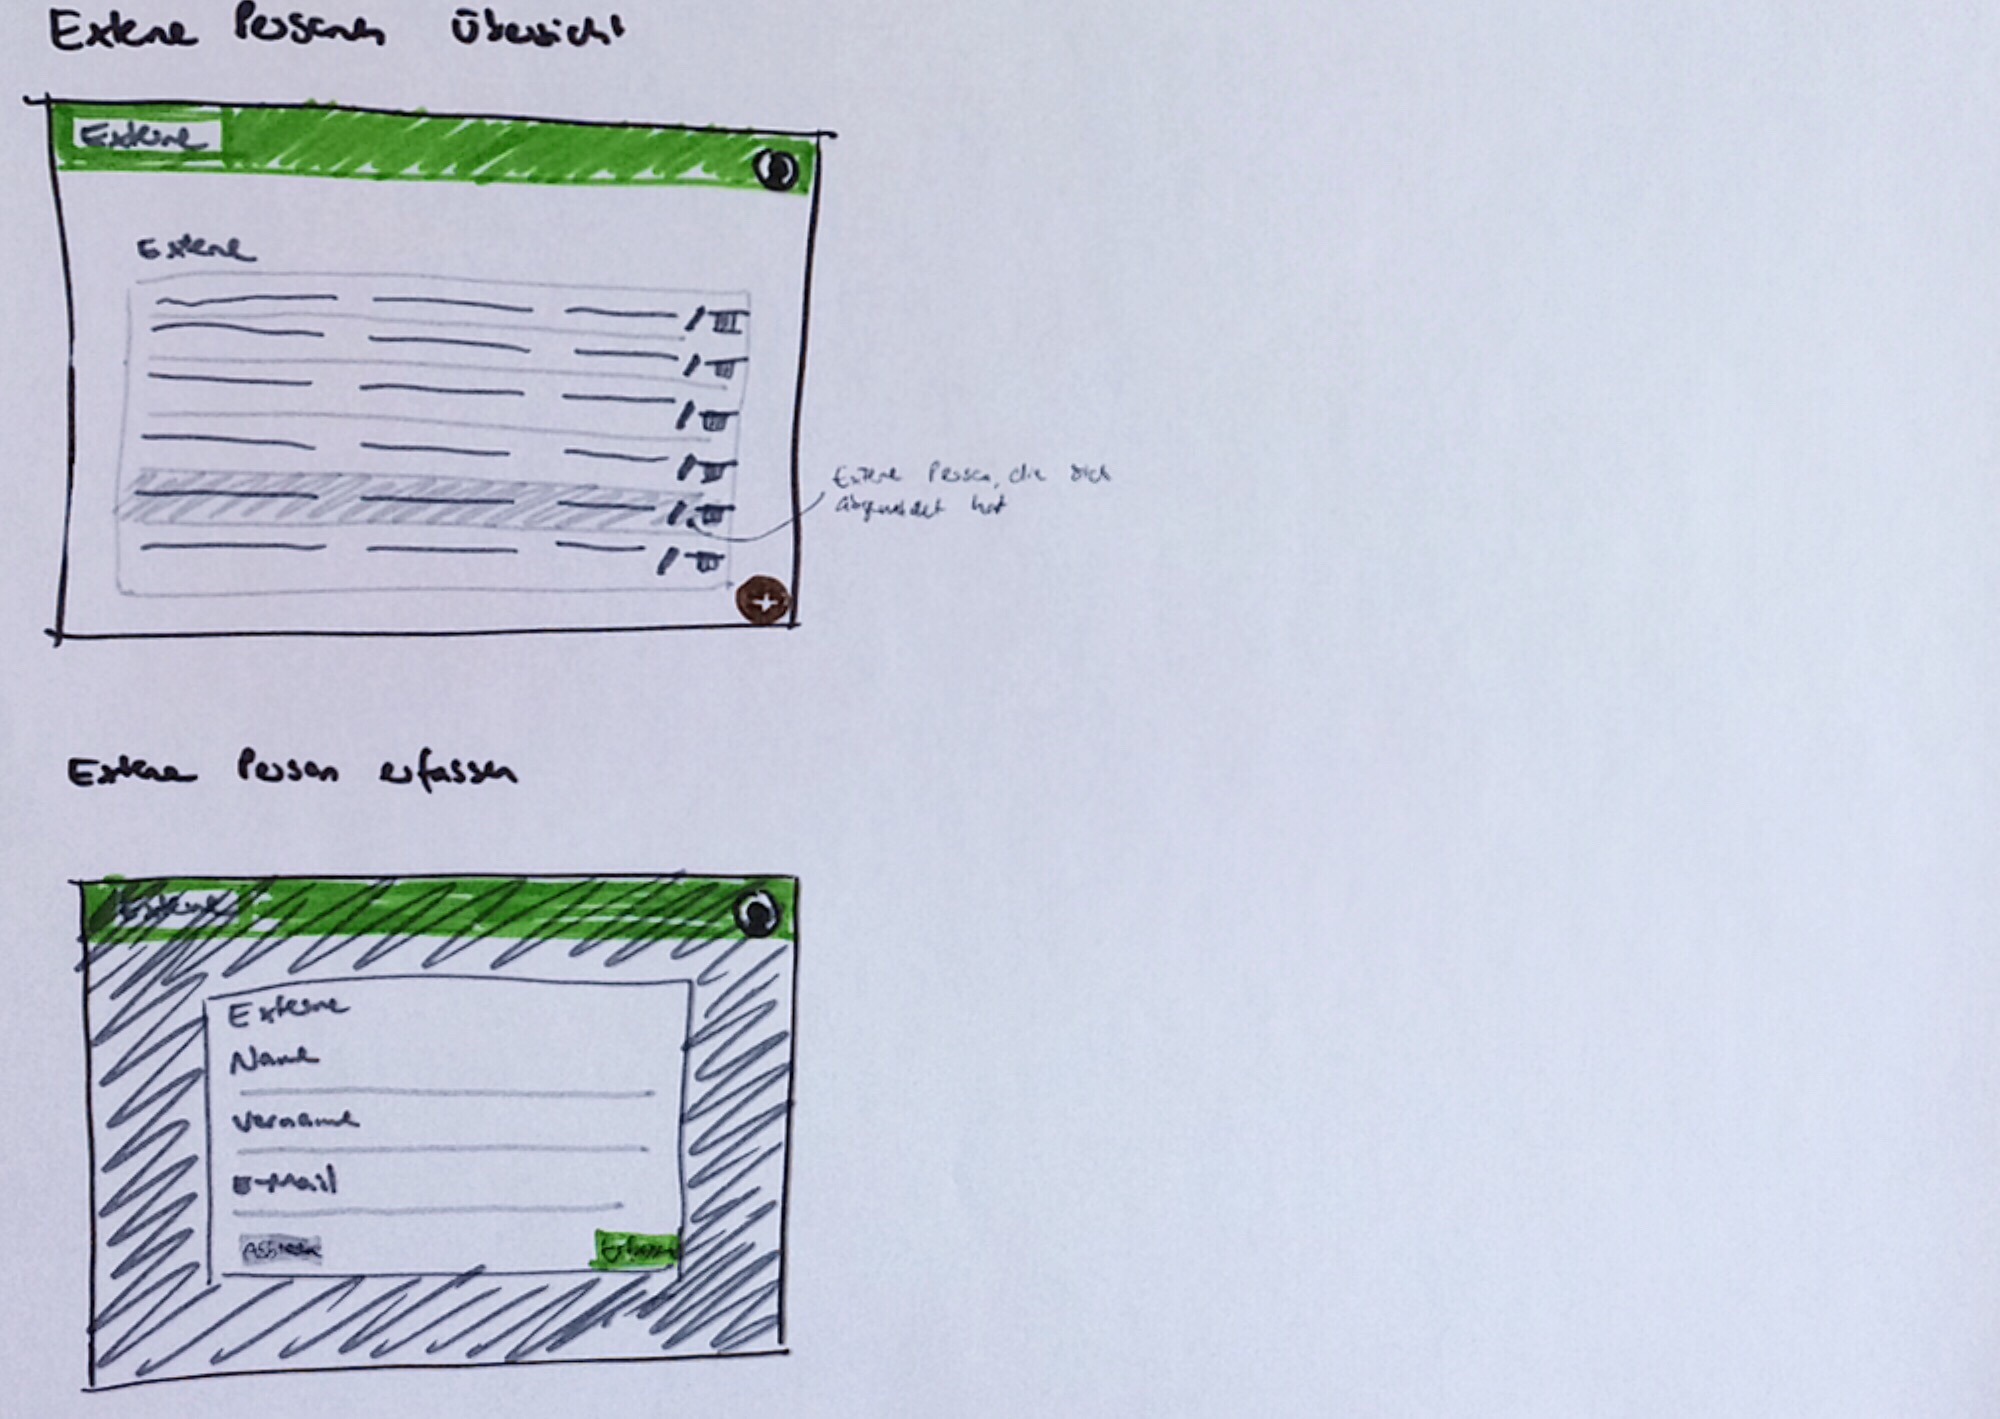
\includegraphics[width=1\textwidth]{prototyp/ExternePersonen}

\subsection{Detailansicht}
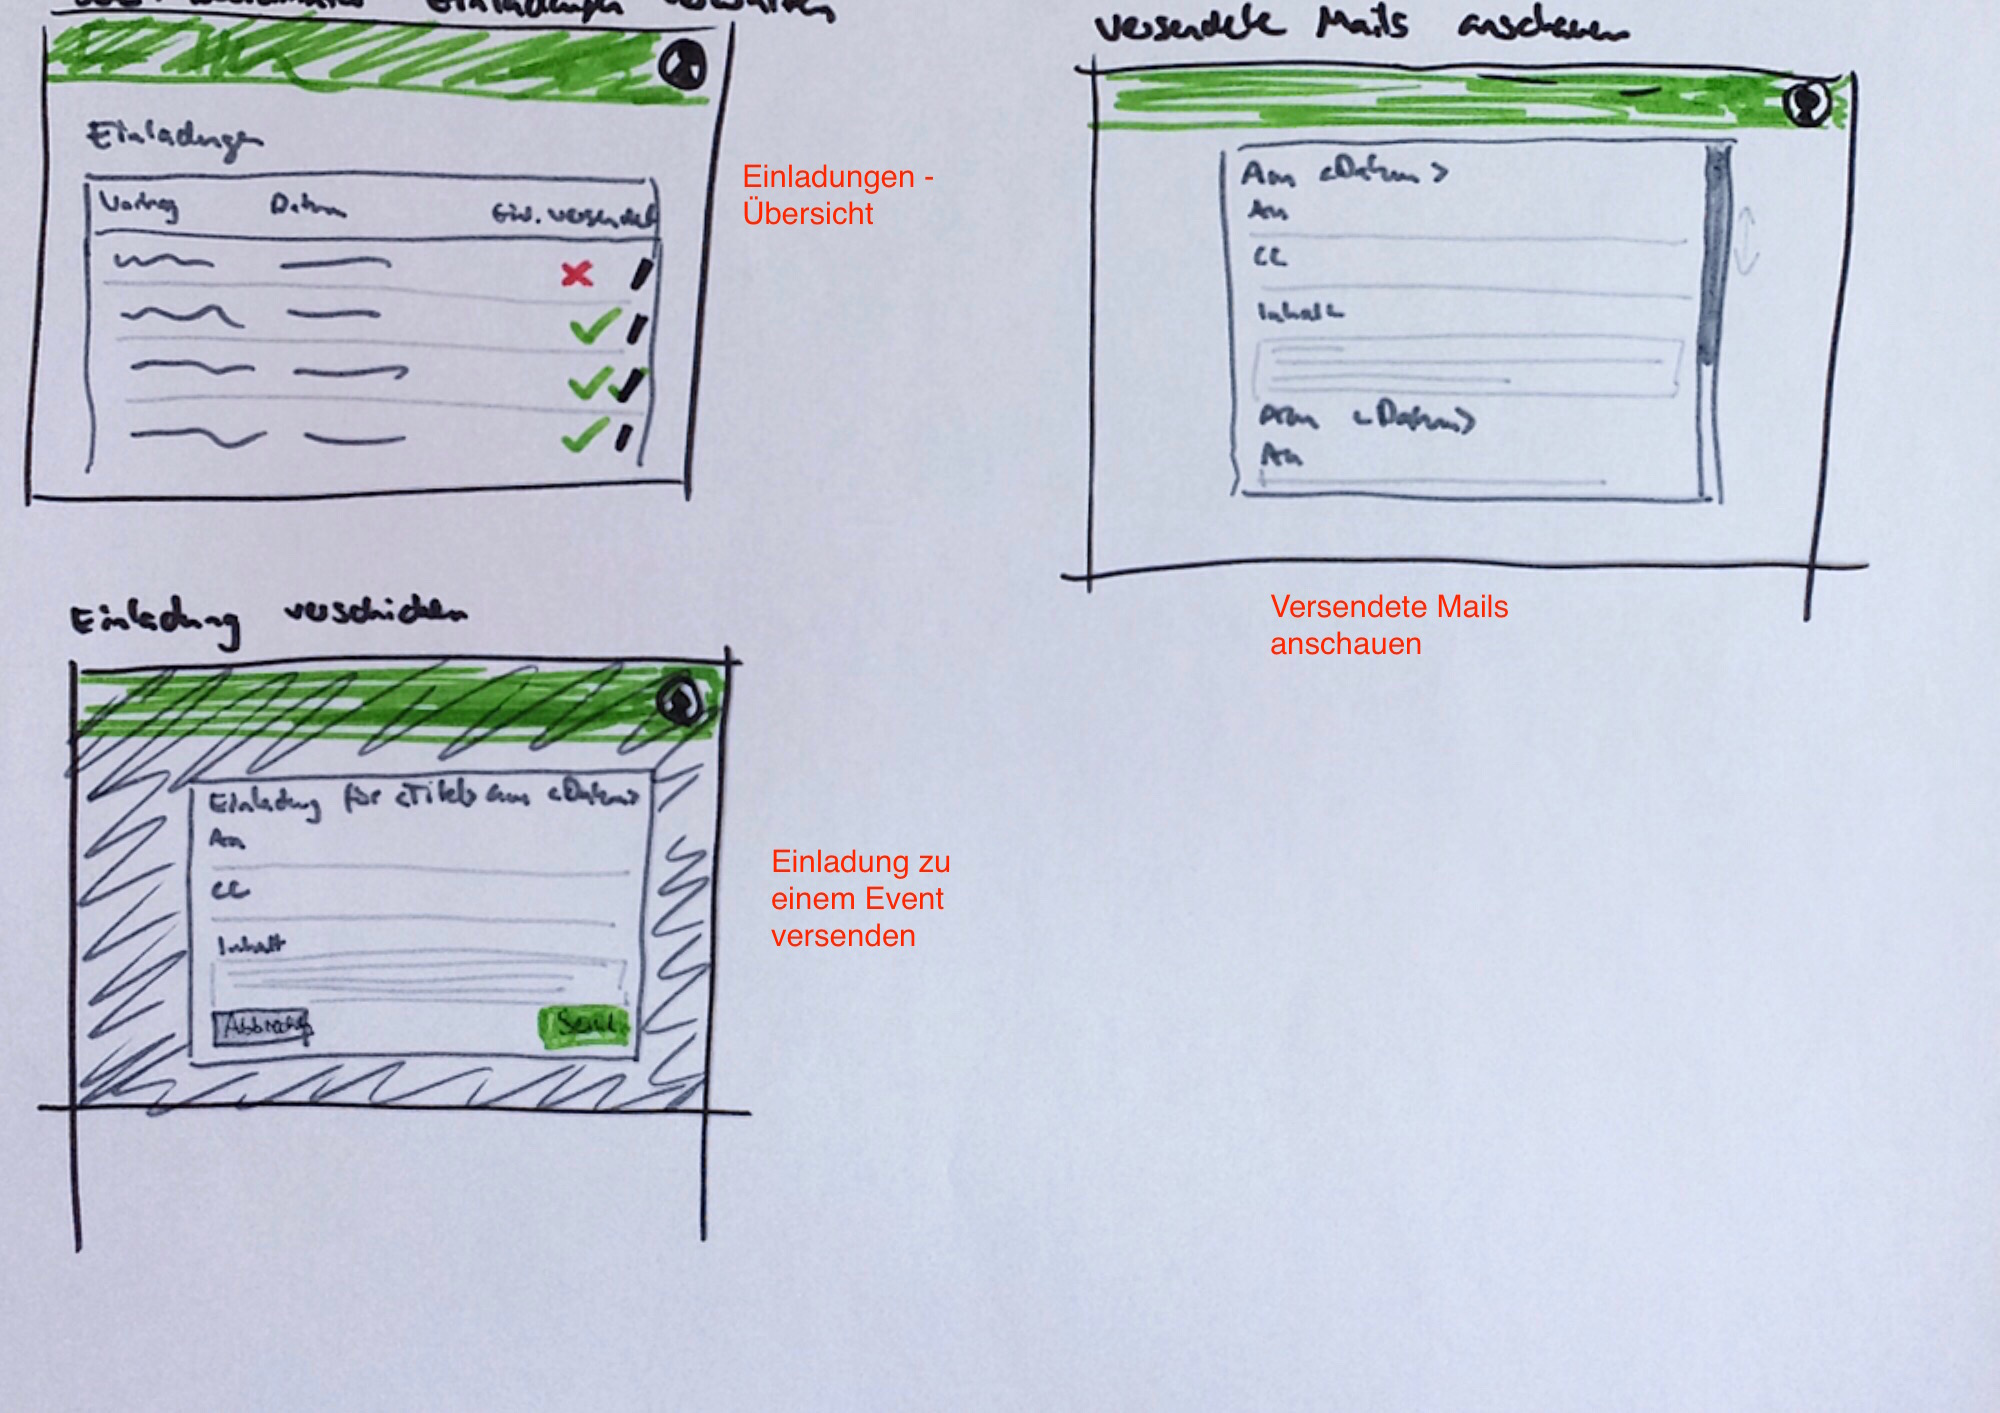
\includegraphics[width=1\textwidth]{prototyp/Einladungen}

\subsection{Einschreiben}
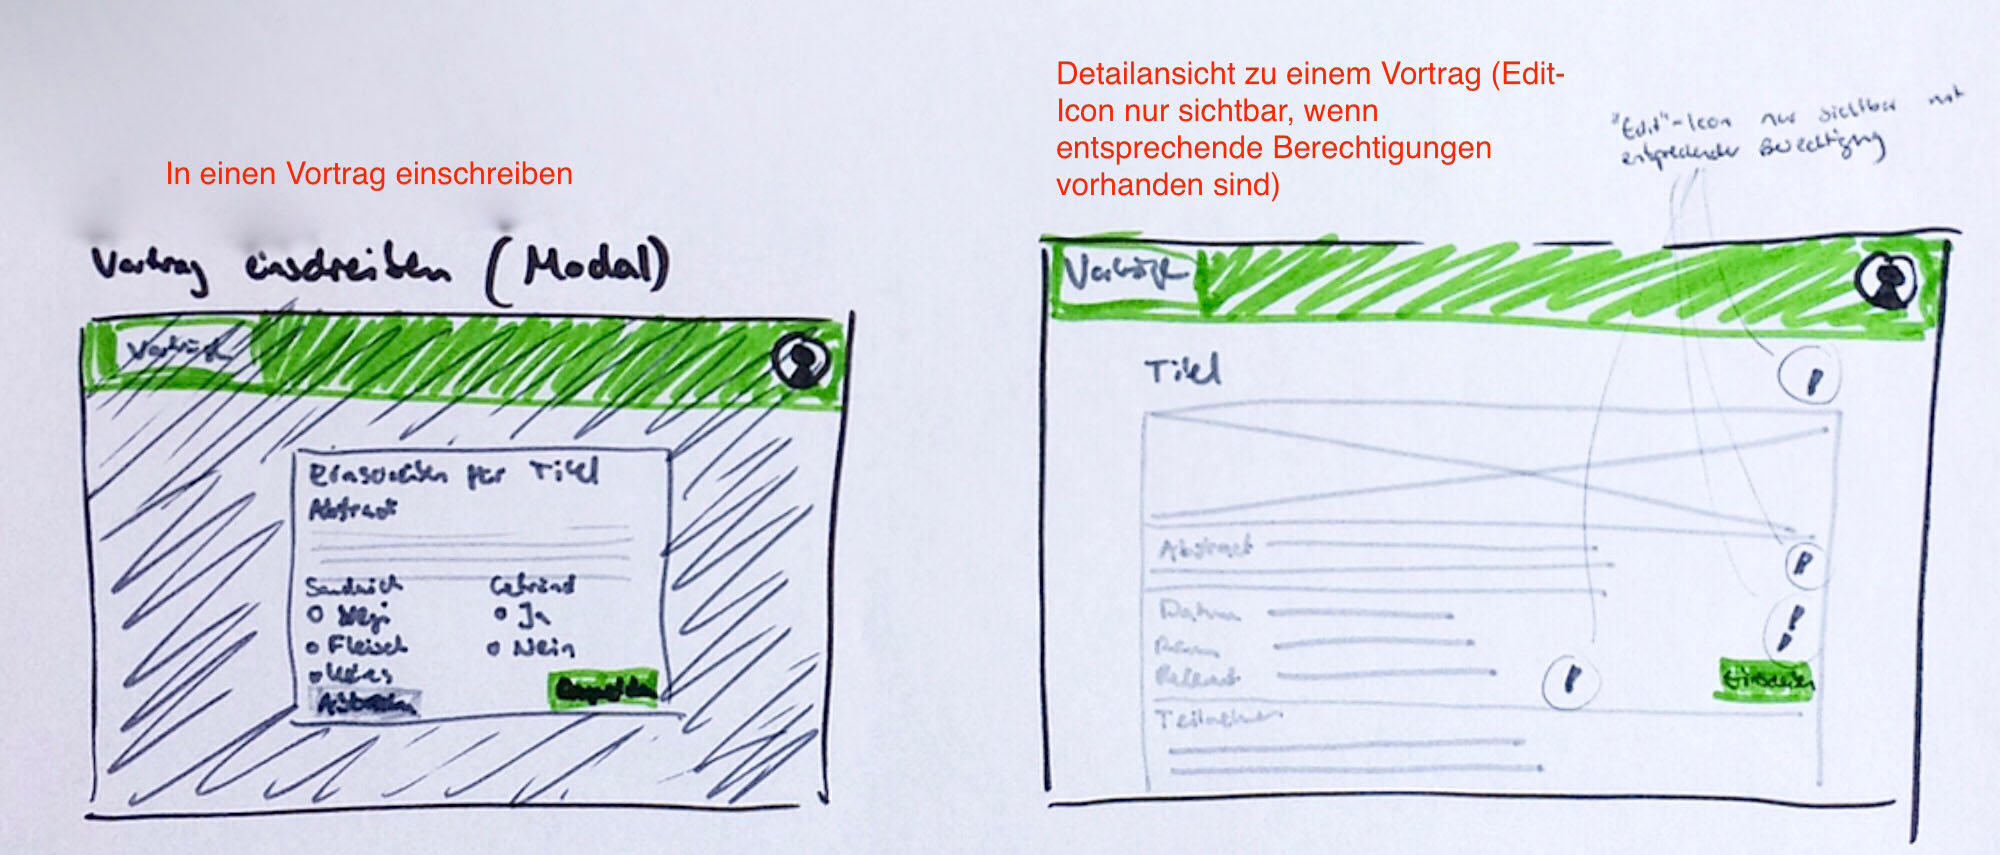
\includegraphics[width=1\textwidth]{prototyp/Vortrag}

\newpage
\section{Architektur}
Unsere Implementation des "Event-Planners" wird als Microservices realisiert. Wir verwenden dazu "Eureka", eine Library entwickelt von Netflix https://github.com/netflix/eureka.  Die Applikation lässt sich in fünf Microservices unterteilen, welche im nachfolgenden Abschnitt genauer beschrieben werden. Die Microservices kommunizieren per REST untereinander.


\subsection{Microservices}
\subsubsection{Registry}
	Das "Bindeglied" zwischen den verschiedenen Microservices. Die Microservices verbinden sich auf die Registry um dort die URLs der anderen Microservices zu bekommen. Dadurch wird es möglich, die Applikation auf mehreren Servern verteilt laufen zu lassen. Im Falle einer bestehenden Eurika Installation/Architektur muss dieser Microservice nicht nochmals zusätzlich gestartet werden (bestehende Registry kann verwendet werden).

\subsubsection{Eventmanagement}
	Beinhaltet alle Entitäten (Persistance Layer) sowie die Businesslogik unserer Applikation und ermöglicht den Zugriff von aussen. Hierfür werden die CRUD Operationen über eine REST-API zur Verfügung gestellt. Bestimmte Endpunkte stehen dabei nur nach erfolgreicher Authentifizierung und Autorisierung zur Verfügung. Die komplette Schnittstellendokumentation ist im Anhang (Swagger Schnittstellendokumentation) aufgeführt.

\subsubsection{Frontend}
	Container welcher nur dazu dient, statische Inhalte zur Verfügung zu stellen. Enthält keinerlei Business Logik. Konkret wird der Build Order unserer Ionic App in den assets/static Order kopiert. Sollte bereits eine bestehende Webserver Infrastruktur zur Verfügung stehen (z.B. Apache oder Nginx), können diese Assets auch ohne zusätzlichen Microservice gehosted werden.

\subsubsection{Mailer}
	Simpler Mailservice, welcher eine API zum Versenden von Mails bietet. Diese API wird durch ein statische Token geschützt, es werden ausschließlich interne (von anderen Microservices) Anfragen entgegengenommen.

\subsubsection{Scheduler}
	Scheduler Service, welcher zu bestimmten Zeiten Tasks ausführt. Ein Beispiel hierfür wäre, unreferenzierte  Mediendateien in der Nacht zu löschen, Erinnerungsmails zu versenden oder Events aufgrund verschiedener Kriterien zu archivieren.

\newpage
\subsection{Datenbank}
Um für die Datenintegrität garantieren zu können, werden alle Entitäten durch einen einzigen Microservice verwaltet (https://www.nginx.com/blog/microservices-at-netflix-architectural-best-practices/).

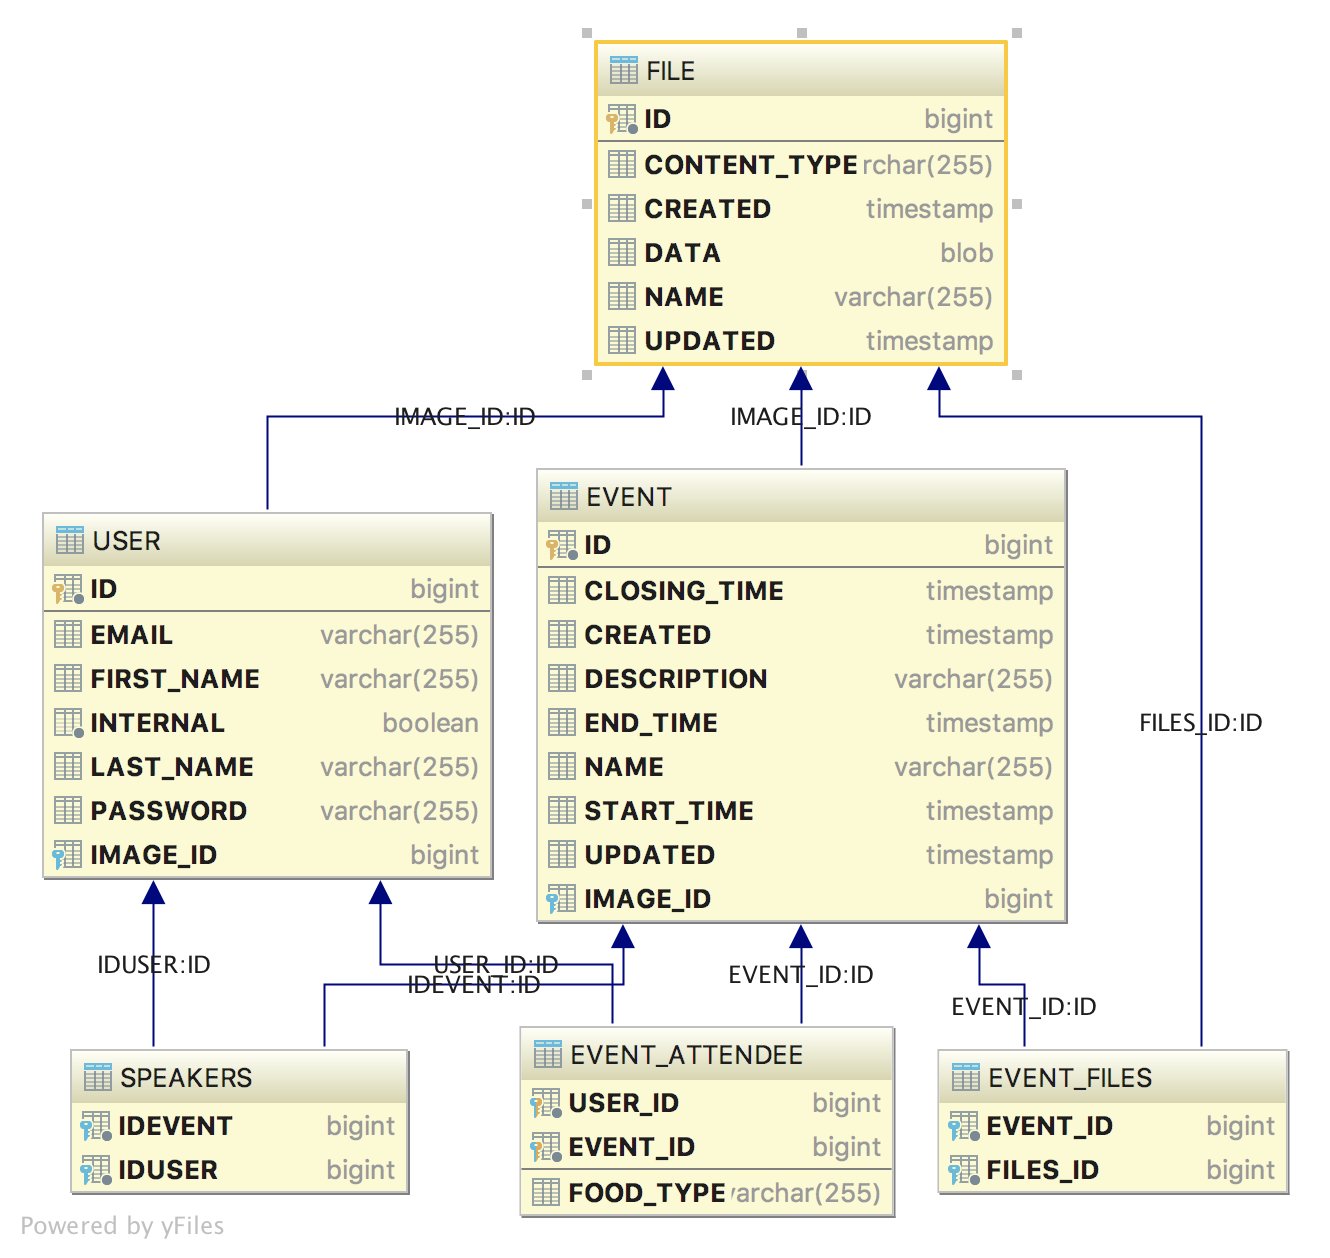
\includegraphics[width=1\textwidth]{dbSchema}

\newpage
\section{Technology}

\subsection{Frontend}
Nach dem Start mit Angular 2 merkten wir schnell, das uns einige Standardkomponenten fehlten. Außerdem war der Aufwand die Seite Mobile tauglich zu machen größer als erwartet. Aus diesem Grund wechselten wir nach kurzer Zeit auf Ionic 2. Da Ionic 2 auf Angular 2 aufbaut, war der Wechsel schnell vonstatten gegangen. Mithilfe der neuen Sidemenu Komponente kann die Webseite ohne weitere Probleme für Desktops optimiert werden.

\subsection{Backend}
Wie von der Projektbeschreibung vorgeschrieben, verwenden wir Java mit Spring Boot im Backend. Zusätzlich verwenden wir die spring-boot-data Erweiterung, welche uns das einfache erstellen von Rest Repositories ermöglicht. 

\subsubsection{Autentifizierung und Autorisierung}
Für die Authentifizierung verwenden wir PAC4J und verwenden das JWT (Json Web Token). Zusätzlich können mithilfe von PAC4J Permissions und Rollen definiert werden. Abhängig von der Rolle, erhält der Benutzer zusätzliche Privilegien. Ein normaler Besucher kann lediglich Events ansehen und nichts editieren. Wir haben folgende Rollen identifiziert:

\begin{enumerate}
\item Besucher
\item Angemeldeter Gast (kann sich zusätzlich einschreiben)
\item Referent (kann zusätzlich den eigenen Event bearbeiten und Dateien anhängen)
\item Koordinator (kann alle Entitäten bearbeiten und löschen)
\end{enumerate}



\newpage
\begin{appendices}

\textbf{Swagger Schnittstellendokumentation}\\
\url{https://htmlpreview.github.io/?https://raw.githubusercontent.com/lukeisontheroad/simple_event_planner/master/docs/doc.html}\\

\textbf{Github Repository}\\
\url{https://github.com/lukeisontheroad/simple_event_planner}\\

\textbf{Microservices best practices}\\
\url{https://www.nginx.com/blog/microservices-at-netflix-architectural-best-practices/}\\

\textbf{PAC4J}\\
\url{http://www.pac4j.org/}\\



\newpage

\end{appendices}

\end{document}
